\chapter{Following the path}
\label{ch:following}

A plan is a promise about where the mower will be. On a real machine, a
controller turns the steering so that the mower follows the planned path,
using an estimate of where it is. That estimate has errors, the steering
takes time to turn, and the mower drifts from the path. This chapter
simulates that loop and measures what it does to the result: how far the
mower strays, what it leaves uncut, and when it touches the border.

\section{The loop}

The simulation repeats, every $\Delta t = \SI{20}{\milli\second}$:

\begin{description}
  \item[Localisation.]
    \leavevmode\\
    Every \SI{0.1}{\second}, a new estimate of the pose arrives: the true
    pose plus Gaussian errors, of standard deviation $\sigma_p$ on each
    coordinate and $\sigma_\theta$ on the heading. Satellite positioning
    with corrections (RTK) gives about \SI{2}{\centi\metre}; without
    corrections, a metre or more. In between, the estimate is carried
    forward by the motion the mower knows it has made (odometry).
  \item[Control.]
    \leavevmode\\
    The controller compares the estimate with the path and asks for a
    curvature, hence a steering angle.
  \item[Steering.]
    \leavevmode\\
    The steering turns towards that angle at most at the rate $\omega$
    (Chapter~\ref{ch:smooth}).
  \item[Motion.]
    \leavevmode\\
    The mower drives $v\,\Delta t$ on the arc of its current curvature,
    at the speed of the plan at the closest point of the path.
\end{description}

The path is driven piece by piece between its changes of direction: at
the end of a piece, the mower stops, waits $t_{\mathrm{shift}}$ and turns
the steering towards the start of the next piece while standing. The
executed motion is again a list of short arcs, measured as any plan.

\section{Feedback with feedforward}

Let $s$ be the distance along the path, $e_y$ the signed distance from the
rear axle to the closest point of the path (positive to the left of the
direction of travel), and $e_\theta$ the heading of the mower minus that of
the path there. For a mower close to the path, driving a distance $ds$
changes them by
\[
  \frac{de_y}{ds} = \sin e_\theta \approx e_\theta, \qquad
  \frac{de_\theta}{ds} = \kappa - \kappa_{\mathrm{ref}},
\]
where $\kappa$ is the curvature the mower drives and
$\kappa_{\mathrm{ref}}$ that of the path (both counted along the direction
of travel).

\begin{proposition}{A critically damped correction}{feedback}
  The control
  \[
    \kappa = \kappa_{\mathrm{ref}} - \frac{e_y}{\ell^2}
      - \frac{2 \sin e_\theta}{\ell}
  \]
  gives, for small errors, $e_y(s) = \bigl(e_0 + (e_0/\ell + e'_0)\,s\bigr)
  e^{-s/\ell}$, where $e_0$ and $e'_0$ are the error and its slope at $s =
  0$: the error dies out over a few times the distance $\ell$, without
  overshoot.
\end{proposition}

\begin{proof}
  Differentiating $de_y/ds \approx e_\theta$ and substituting the control,
  \[
    \frac{d^2 e_y}{ds^2} = \kappa - \kappa_{\mathrm{ref}}
    = -\frac{e_y}{\ell^2} - \frac{2}{\ell}\frac{de_y}{ds}.
  \]
  The characteristic equation $r^2 + 2r/\ell + 1/\ell^2 = 0$ has the double
  root $r = -1/\ell$, so $e_y = (A + Bs)e^{-s/\ell}$; the initial
  conditions give $A = e_0$ and $B - A/\ell = e'_0$.
\end{proof}

The term $\kappa_{\mathrm{ref}}$ (\emph{feedforward}) steers the curvature
of the path before any error appears; the two others (\emph{feedback})
correct the errors. The distance $\ell$ sets how firmly: a short $\ell$
corrects fast but asks the steering for quick changes that its rate limit
cannot follow, and amplifies the noise of the estimate; the code uses
$\ell = \SI{1}{\metre}$. The same law holds in reverse: the curvature of the
path of the rear axle is set by the steering in the same way whichever way
the mower drives, so only the direction of travel changes.

\section{Pure pursuit}

A classic alternative, \emph{pure pursuit}~\cite{coulter1992implementation}, aims at
the point of the path a lookahead distance $L_d$ ahead of the closest one,
and drives the arc that reaches it.

\begin{proposition}{The arc through the goal point}{purepursuit}
  If the goal point is at the distance $D$ from the rear axle and at the
  lateral offset $y_g$ from the direction of travel, the arc that starts
  along the direction of travel and passes through it has curvature
  $\kappa = 2 y_g / D^2$.
\end{proposition}

\begin{proof}
  The centre of the arc is on the lateral axis, at $(0, 1/\kappa)$ in the
  frame of the mower. The goal $(x_g, y_g)$ is on the circle:
  $x_g^2 + (y_g - 1/\kappa)^2 = 1/\kappa^2$, that is $x_g^2 + y_g^2 =
  2 y_g/\kappa$, and $x_g^2 + y_g^2 = D^2$.
\end{proof}

Pure pursuit needs no curvature of the path, only points of it, which makes
it robust; but it starts turning when the goal point enters a bend, before
the mower reaches it, and so cuts the inside of every bend.
Figure~\ref{fig:controllers} compares the two on a forward turn.

\begin{figure}[ht]
  \centering
  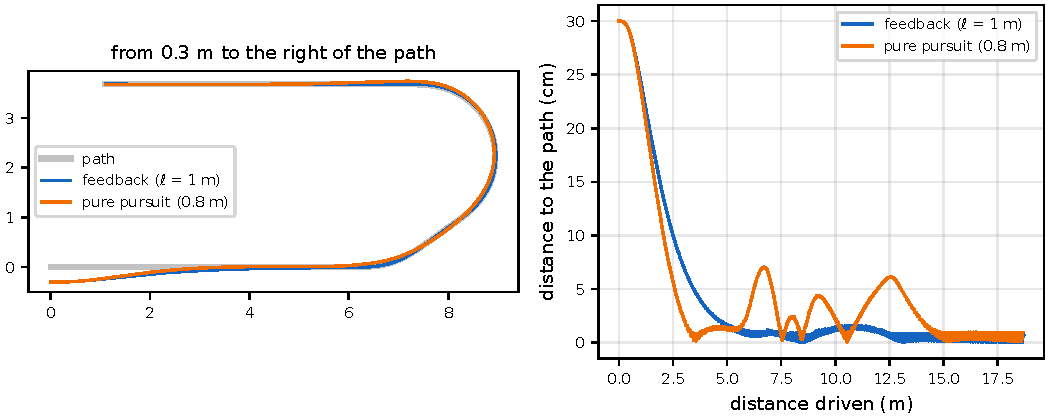
\includegraphics[width=\textwidth]{figures/controllers}
  \caption{The two controllers on a straight line, a forward turn with
    ramps four passes over, and a straight line, starting
    \SI{0.3}{\metre} to the right of the path, with an exact estimate of
    the pose. Left: the paths. Right: the distance to the path. Feedback
    with feedforward converges as in Proposition~\ref{prop:feedback} and
    stays within \SI{2}{\centi\metre} through the turn; pure pursuit
    converges faster here, but cuts the turn by up to
    \SI{7}{\centi\metre}.}
  \label{fig:controllers}
\end{figure}

\section{Errors and their effects}

The plan of the rectangle with ramps (Chapter~\ref{ch:smooth}) was driven
by both controllers with four levels of localisation error, three times each
with different random errors; the table gives the averages. The distance to
the path is measured from the rear axle to the planned path.

\begin{center}
\begin{tabular}{@{}lrrrrrr@{}}
  \toprule
  controller & $\sigma_p$ & $\sigma_\theta$ & rms & 95\% & largest
    & collisions \\
  \midrule
  feedback & 0 & 0 & \SI{1.0}{\centi\metre} & 2.2 & 3.4 & 0 \\
  feedback & \SI{2}{\centi\metre} & $0.5°$ & 2.3 & 4.5 & 10.3 & 0 \\
  feedback & \SI{5}{\centi\metre} & $1°$ & 5.7 & 11.3 & 28.0 & 62 \\
  feedback & \SI{10}{\centi\metre} & $2°$ & 9.8 & 19.8 & 52.5 & 182 \\
  pure pursuit & 0 & 0 & 6.9 & 9.2 & 54.8 & 0 \\
  pure pursuit & \SI{2}{\centi\metre} & $0.5°$ & 5.6 & 10.0 & 37.6 & 0 \\
  pure pursuit & \SI{5}{\centi\metre} & $1°$ & 11.7 & 21.7 & 73.3 & 68 \\
  pure pursuit & \SI{10}{\centi\metre} & $2°$ & 16.6 & 35.1 & 84.3 & 255 \\
  \bottomrule
\end{tabular}
\end{center}

The distances are in centimetres; collisions count the samples of the
executed path where the mower's outline enters the margin of
\SI{5}{\centi\metre} along the border. The plan cuts 89.4\% of the lawn in
\SI{6.31}{\minute}; every executed path cuts between 88.3\% and 90.2\%, in
6.30 to \SI{6.47}{\minute}.

\begin{description}
  \item[Without errors,]
    \leavevmode\\
    the feedback controller stays within \SI{3.4}{\centi\metre} of the
    path: the path with ramps is one the steering can follow. Pure pursuit
    strays by up to \SI{55}{\centi\metre}, in the short pieces of the
    manoeuvres, where the goal point runs past the end of the piece.
  \item[With satellite positioning with corrections]
    \leavevmode\\
    ($\sigma_p = \SI{2}{\centi\metre}$, $\sigma_\theta = 0.5°$), the
    feedback controller stays within \SI{10}{\centi\metre}, and the mower
    never enters the margin.
  \item[With errors of \SI{5}{\centi\metre} and more,]
    \leavevmode\\
    the largest deviations reach \SI{28}{\centi\metre}, and the mower enters
    the margin of \SI{5}{\centi\metre} near the border: the margin must
    then be as large as the largest error, which means a wider uncut strip
    along the border.
\end{description}

The coverage hardly changes, and even grows a little: the wandering passes
cut some of the strip along the border that the plan leaves. The raster of
\SI{5}{\centi\metre} cannot see the thinner gaps that open between two
passes; a simple model estimates them.

\begin{proposition}{Gaps between passes}{gaps}
  If the lateral errors of two neighbouring passes are independent, normal,
  with mean $0$ and standard deviation $\sigma_e$, a gap opens between them
  where their difference exceeds the overlap $o$, which happens along a
  fraction
  \[
    P = \Phi\Bigl(-\frac{o}{\sqrt 2\, \sigma_e}\Bigr)
  \]
  of their length, where $\Phi$ is the standard normal distribution
  function. To keep this fraction below $P$, the overlap must be at least
  $o = \sqrt 2\, \sigma_e\, z_P$, with $\Phi(-z_P) = P$.
\end{proposition}

\begin{proof}
  The two passes are $s = w - o$ apart, and their cuts meet as long as the
  distance between them stays below $w$, that is as long as their errors
  move them apart by less than $o$. The difference of two independent
  normal errors is normal with standard deviation $\sqrt 2\,\sigma_e$, and
  it exceeds $o$ with the probability $\Phi(-o/(\sqrt 2\,\sigma_e))$.
\end{proof}

\begin{example}{The overlap the errors need}{overlap}
  With $\sigma_e = \SI{2.3}{\centi\metre}$ (corrected positioning) and $o =
  \SI{5}{\centi\metre}$, $P = \Phi(-5/(1.414 \times 2.3)) = \Phi(-1.54) =
  \SI{6}{\percent}$ of the length has a gap, mostly of a centimetre or two.
  With $\sigma_e = \SI{5.7}{\centi\metre}$, $P = \Phi(-0.62) =
  \SI{27}{\percent}$. To bring the fraction down to \SI{1}{\percent}
  ($z_P = 2.33$), the overlap must be $1.414 \times 2.33 \times \sigma_e =
  3.3\,\sigma_e$: \SI{7.6}{\centi\metre} with corrected positioning,
  \SI{19}{\centi\metre} without.
\end{example}

Errors at successive points of a pass are not independent (the controller
smooths them over about $\ell$), so the gaps come in streaks rather than
scattered points, but their total length follows the same fraction.
Figure~\ref{fig:following} shows one of the runs with errors of
\SI{5}{\centi\metre}.

\begin{figure}[ht]
  \centering
  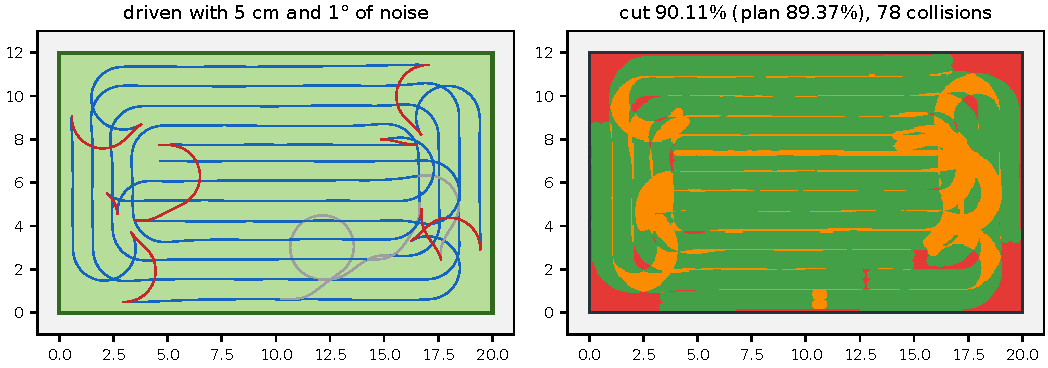
\includegraphics[width=\textwidth]{figures/following}
  \caption{The plan of the rectangle with ramps, driven by the feedback
    controller with localisation errors of \SI{5}{\centi\metre} and $1°$.
    Left: the executed path (blue forward, red reverse, grey blades off).
    Right: the grass cut (green once, orange twice, red missed). The passes
    wander by a few centimetres; near the border the mower enters the margin
    in a few places.}
  \label{fig:following}
\end{figure}

\begin{inwords}
  A controller that steers the curvature of the path and corrects the
  errors gently follows a path with ramps within a few centimetres. With
  satellite positioning with corrections, the noise of the estimate costs
  little; with a less precise estimate, the passes wander, gaps open
  between them, and the mower comes closer to the border than planned. The
  overlap between passes and the margin to the border are the insurance
  against these errors, and their size follows from the size of the errors.
\end{inwords}

\begin{incode}
  \code{mowersim/follow.py}: \code{Follower} (the settings),
  \code{pieces} (the path cut at the changes of direction) and
  \code{follow} (the loop, both controllers). From the command line:
  \begin{verbatim}
python -m mowersim plan lawns/rectangle.json --smooth --follow 0.05
  \end{verbatim}
\end{incode}
